\ifx\master\undefined\input{settings/autocompile}\fi
\chapter{The Compact Muon Solenoid Experiment}
\label{ch:detector}
%

The Compact Muon Solenoid (CMS) Experiment is a ``general purpose'' particle
detector designed to measure collision events at the Large Hadron Collider
(LHC), a proton--proton synchrotron located at the CERN laboratory in Geneva,
Switzerland.  The design goals of the CMS experiment are~\cite{CMSExperiment},
in order of priority:
\begin{itemize}
  \item Good muon identification and momentum resolution over a wide range of
    momenta and angles, good dimuon mass resolution ($\approx 1\%$ at 100~\GeV),
    and the ability to determine unambiguously the charge of muons with $p <
    1~\TeV$;
  \item Good charged-particle momentum resolution and reconstruction efficiency
    in the inner tracker. Efficient triggering and offline tagging of $\tau$'s and
    $b$--jets, requiring pixel detectors close to the interaction region;
  \item Good electromagnetic energy resolution, good diphoton and dielectron
    mass resolution ($\approx 1\%$ at 100~\GeV), wide geometric coverage,
    $\pi^0$ rejection, and efficient photon and lepton isolation at high
    luminosities;
  \item Good missing--transverse--energy and dijet--mass resolution, requiring
    hadron calorimeters with a large hermetic geometric coverage and with fine
    lateral segmentation.
\end{itemize}
The detector uses a hermetic design that maximizes the
solid--angle of the fiducial region to capture as much information about the
collisions as possible.  The general geometry of the detector is cylindrical.
At cutaway diagram of the detector is shown in Figure~\ref{fig:AllCMSCutaways}.
Each of the sub--detector components consists of ``barrel'' and ``endcap''
components.  As its name suggests, the detector is centered around a four Tesla
superconducting solenoid magnet.  The individual sub--detectors of CMS are
arranged in a manner that permits identification of different species of
particles.  The central (closest to interaction point) sub--detector are the
charged particle tracking systems (the ``tracker'').  The tracker is designed to
be a \emph{non--destructive} instrument, which means that ideally that the
momentum of particles are unchanged after passing through it.  Outside of the
tracker is the electromagnetic and hadronic calorimeters, which are abbreviated
ECAL and HCAL, respectively.  The calorimeter is a \emph{destructive} detector,
and is designed such that visible incident particles are completely absorbed.
The outer layers of CMS are designed to measure muons, the
one\footnote{Neutrinos of course fulfill this requirement as well, but are so
weakly interacting that they are effectively invisible.} species of particle
that is immune to the effects of the calorimeter.  The arrangement of
destructive and non--destructive sub--detectors facilitates the identification
of different types of particles.  This concept is illustrated in
Figure~\ref{fig:SubdetectorID}.
\begin{figure}
  \centering
  %\subfigure[]{\includegraphics[width=0.97\textwidth]{detector_chapter/figures/cms_complete_labelled.pdf}
  \subfigure[]{\includegraphics[width=0.97\textwidth]{detector_chapter/figures/cms_complete_labelled.png}
  \label{fig:CMSDetector}
  }
  \subfigure[]{\includegraphics[width=0.97\textwidth]{detector_chapter/figures/CMS_Slice.png}
  \label{fig:SubdetectorID}
  }
  \caption[Schematic drawings of the CMS
  detector]{Figure~\subref{fig:CMSDetector}, top, shows a schematic drawing of the CMS
  detector.  The individual sub--detectors are labeled.  Two humans are shown in
  the foreground for scale. Figure~\subref{fig:SubdetectorID} shows a radial
  cross section of the detector and demonstrates how
  the (non--)destructiveness of different sub--detectors facilitates particle
  identification.} 
  \label{fig:AllCMSCutaways}
\end{figure}
In this chapter we give an brief overview of the LHC machine, and then describe
the individual sub--detector systems of CMS. 

\section{The Large Hadron Collider}
The Large Hadron Collider is a proton--proton synchrotron, with a design
collision energy of 14~\TeV.  At the time of this writing (and for the
foreseeable future), the LHC is the world's largest and highest energy particle
accelerator. A synchrotron is a machine that accelerates beams of charged
particles by using magnets to steer them in a circle through radio--frequency
resonating cavities which accelerate the particles. As the LHC is a collider,
there are two beams that are accelerated in opposite directions.  The maximum
beam energy of a synchrotron is determined by its radius and the maximum
strength of the magnetic fields used to bend the path of the beam.  The dipole
magnets used by the LHC to steer the particles are superconducting
niobium--titanium.  To maintain them in a superconducting state, they are cooled
using superfluid liquid helium to 1.9~Kelvin.  To store the beam at the
injection energy of 450~\GeV, the magnetic dipole fields must be maintained at
$1/2$~Tesla.  As the energy of each beam energy is increased to its (design)
maximum of 7~\TeV, the dipole fields are ramped to a maximum field of over 8
Tesla.
\section{Solenoid Magnet}
\label{sec:Magnet}
The four Tesla field of the CMS solenoid magnet is a critical factor in ability
of CMS to precisely measure collisions at the LHC\@. The momentum of charged
particles is measured in the detector by examining the curvature of the
particles path as it travels through the magnetic field.  The radius of
curvature $r$ of a charged particle in a magnetic field is given by
\begin{equation}
  r = \frac{p_\perp}{|q| B},
  \label{eq:LarmorRadius}
\end{equation}
where $q$ is the charge of the particle, $B$ is the magnetic field, and
$p_\perp$ is the component of the particle's relativistic momentum perpendicular
to the direction of the magnetic field.  From Equation~\ref{eq:LarmorRadius}, it
is evident that the ability to measure high momentum charged particles (a
critical goal of CMS) requires a high magnetic field.  Even at very high
particle energies where the resolution becomes poor, the strength of the
magnetic field is still very important for identifying the bending direction of
the particle; the direction corresponds to the particle's electric charge.
Furthermore, the homogeneity of the magnetic field is important to minimize
systematic errors in the measurement of tracks.

The CMS solenoid is extremely large.  The radial bore of the magnet is
6.3~meters; the magnet is 12.5~meters in length and weighs 220~tons.  The large
bore of the magnet allows the tracker and calorimeter systems to be located
inside the solenoid.  The internal windings of solenoid is arranged in four
layers to increase the total field strength and are cooled by liquid helium to
a temperature of 4.5 Kelvin.  The windings are magnetically
coupled to the support superstructure.  This coupling allows the magnetic to
heat uniformly during a ``quench\footnote{A quench event occurs when some part
of the magnet is suddenly no longer in a superconducting state.  The coil
becomes resistive and the large current in the magnet creates large amounts of
heat.}'' event, reducing localized stresses.  The
nominal current at full field of the solenoid is 19.14~kA.  The solenoid itself
is surrounded by an iron return yoke with a total mass of 10,000~tons.  The
return yoke surrounding the solenoid minimizes the fringing field.  The muon
detector system is interspersed inside the yoke, and takes advantage of the
field in the yoke to measure the momentum and charge of muons.
%
\section{Charged Particle Tracking Systems}
\label{sec:Tracker}

The charged particle tracking system measures the trajectories of charged
particles emerging from the event.  The tracker measures the trajectory of a
charged particle by measuring ``hits'' along the trajectory.  Each hit
corresponds to the global position of the trajectory on a given surface.  The
trajectory can then be reconstructed by a helix to the points.  The tracker is
designed to have a resolution that permits the reconstruction of ``secondary
vertices'' in $b$--quark and $\tau$ lepton decays.  To accomplish this, there
are two types of tracking detectors in CMS\@.  The ``pixel detector''composes
the inner layers (three in the barrel, two in the endcaps).  The pixel detector
is  situated as close as possible (4.4~\cm) to the interaction point and has a
very high resolution. Outside of the pixel detector is the silicon strip
tracker, with ten layers in the barrel and 12 layers in the endcaps.  A
secondary vertex occurs when a particle is semi--stable, traveling some
non--negligible distance in the detector, but decaying before the first layer of
the tracking system.  The pixel and strip tracking detectors have a fiducial
region which extends to a pseudorapidity of approximately $|\eta| \approx 2.5$.

Both the pixel and strip trackers are silicon based.  The principle of operation
is similar to that of a charged--coupled discharge (CCD) \fixme{right acronym}
in a modern digital camera.  The sensitive portion of the detector is a silicon
chip that is arranged with diode junctions formed by a $p$--doped layer and an
$n$--doped layer\footnote{The pixel detector actually uses a more complicated
multi--layered scheme to improve radiation hardness.  For details, see
Section~3.2.2 of~\cite{CMSExperiment}.}.  Each $p-n$ junction is electrically
isolated from adjacent layers. The size of each junction region determines the
spatial resolution of the sensor.  The rear side of the chip is mounted to read--out
electronics.  During operation, a high--voltage reverse bias is applied to each
$p-n$ junction to achieve full depletion.  When a charged particle passes
through the detector, the diode--junction breaks down and the readout system
registers the hit.

The tracking system has been specifically designed for the high radiation
environment around the interaction point.  The detector is cooled to -27\celsius
during operation to minimize damage. Radiation exposure produced in LHC
collisions can change behavior of the tracking detector in three ways.  Over
time, radiation can induce positive holes in oxide layers fond in the read--out
electrons which increase the signal--to--noise ratio.  In the sensor mass
itself, radiation damage changes the doping from $n$ to $p$ over time.  The
required voltage to deplete the sensor will thus increase over time.  The
readout electronics, bias voltage supplies, and cooling systems are designed to
scale with the radiation damage and maintain a signal--to--noise ration of 10:1
or greater for 10 years of LHC operation.  The final radiation effect is not an
integrating effect.  A ``single event upset'' is transient effect where an
ionizing charged particle passes through the readout electronics and changes the
state of the digital circuitry.  

In the ideal case, the tracker would be a non--destructive instrument.  However,
charged particles can interact with the mass of the tracker (and its support
infrastructure).  These interactions limit the resolution of the tracker.  The
amount of matter in the tracker is referred to as the ``material budget''.  The
material budget of the CMS tracker depends heavily on the pseudorapidity $\eta$
and is illustrated in Figure~\ref{fig:TrackerMaterialBudget}.
\begin{figure}
  \centering
  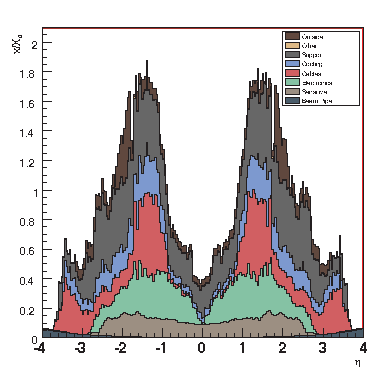
\includegraphics[]{detector_chapter/figures/tracker_material_budget_cleaned.pdf}
  \caption[Material budget of the CMS tracker]{Material budget of the CMS
  tracker in units of radiation lengths $X_0$.  The material budget is broken down
  into the contributions from the different components of the tracker.  The
  amount of material is largest in the ``transition region'' between the barrel
  and endcap.  } \label{fig:TrackerMaterialBudget}
\end{figure}
The relatively large material budget of the CMS tracker has two effects: charged
particles can ``multiple scattering,'' interacting with material in the
tracker.  This can cause ``kinks'' in the reconstructed track.   Hadronic
particles (charged and neutral) can undergo ``nuclear interactions,'' which are
a hard collisions between the incident particle and the tracker material. This
typically produces a spray of hadrons from the point of interaction.  Finally,
the material budget can cause ``photon conversions.''  A photon conversion
occurs when a photon (which typically does not interact with the tracker)
converts into an electron--positron pair while passing through matter in the
tracker.  



\section{Electromagnetic Calorimeter}
\section{Hadronic Calorimeter}
\section{Muon System}
\section{Trigger System}
\section{Particle Flow Reconstruction Algorithm}
\ifx\master\undefined\input{settings/autocompile}\fi
